\documentclass[11pt]{article}

\usepackage[T1]{fontenc}
\usepackage[utf8]{inputenc}
\usepackage[a4paper,margin=24mm]{geometry}
\usepackage{amsmath,amssymb}
\usepackage{booktabs}
\usepackage{graphicx}
\usepackage[table]{xcolor}
\usepackage{tabularx}
\usepackage{microtype}
\usepackage{hyperref}

\hypersetup{
  colorlinks=true,
  linkcolor=blue!45!black,
  citecolor=blue!45!black,
  urlcolor=blue!55!black,
  pdftitle={Explicit-solvent electrostatic dephasing in tandem Venus},
  pdfauthor={Tandem-Venus project}
}

\newcommand{\wn}{\mathrm{cm}^{-1}}
\newcommand{\Ttwo}{T_2^{*}}
\newcommand{\Jmean}{117.19\ \wn}

\title{Explicit-solvent electrostatic dephasing in tandem Venus\\
\large Standalone numerical calculation note}
\author{Tandem-Venus project}
\date{21 July 2026}

\begin{document}
\maketitle

\begin{abstract}
This note records a high-cadence explicit-solvent QM/MM electrostatic-gap test
performed as a sensitivity analysis for the tandem-Venus exciton model.  Two
contiguous 4 ps NVT segments were sampled every 4 fs, and a STEOM-CCSD
excited-minus-ground difference-density probe was used to measure environmental
gap fluctuations at both chromophores.  A classical second-cumulant treatment
gives an inter-site pure-dephasing time of 21.8 fs; an independent OpenMM PME
finite-difference calculation gives 24.0 fs.  The local protein dominates the
differential noise, whereas water is slower and more common-mode.  These values
are useful as a sensitivity bound, but they are not a rigorous quantum-bath
prediction of an experimental coherence time.  The results are deliberately
kept separate from the current manuscript.
\end{abstract}

\noindent\colorbox{yellow!16}{\parbox{0.96\linewidth}{
\textbf{Status.} This is a technical calculation note, not a manuscript
revision.  In particular, the manuscript's phenomenological $\Ttwo=60$ fs
reference has not been replaced by the classical estimate reported here.}}

\section{Question and simulation record}

The calculation asks whether equilibrium fluctuations of the explicit protein,
water and ions can generate dephasing on the same timescale as the solvation
memory used in the physical discussion of tandem Venus.  The retained
full-solvent model contains 69,471 atoms.  Starting from the 1 ns production
checkpoint, two contiguous 4 ps NVT segments were propagated with a 2 fs
timestep.  All atoms were saved every 4 fs, giving 2,000 frames over 7.996 ps.
Both chromophores used the retained AMBER bonded terms and exact anionic CR2
charges.

This trajectory resolves the observed ultrafast decay and permits independent
segment and 1 ps block tests.  It is not long enough to converge slow protein or
bulk-solvent modes.  Consequently, the analysis below is an ultrafast
equilibrium-fluctuation test rather than a complete solvation-response
calculation.

\section{STEOM difference-density probe}

The S1 excited-minus-ground density was reconstructed from all seven printed
STEOM natural-transition-orbital (NTO) pairs.  Their summed represented
occupation is 0.99045993.  Each particle and hole orbital was normalized on its
cube grid before forming
\begin{equation}
  \Delta\rho(\mathbf r)
  = \sum_{k=1}^{7} n_k
    \left(\lvert p_k(\mathbf r)\rvert^2
          -\lvert h_k(\mathbf r)\rvert^2\right).
  \label{eq:difference-density}
\end{equation}
The resulting neutral density was partitioned onto the 41 \emph{physical} QM
atoms.  Hydrogen caps and other link atoms were excluded from the partition and
therefore carry no difference-density charge.  This exclusion is also applied
to density visualizations: the plotted probe contains only physical atoms.

For a chromophore site $m\in\{A,B\}$, the environmental contribution to the
vertical gap was evaluated as
\begin{equation}
  \delta E_m(t) = \sum_{i\in\mathrm{probe}} q_i^{\Delta}
                         \Phi_{\mathrm{MM}}(\mathbf r_{mi},t),
  \label{eq:gap}
\end{equation}
where $q_i^{\Delta}$ is the atom-partitioned difference charge and
$\Phi_{\mathrm{MM}}$ is the instantaneous electrostatic potential from the
explicit environment.  The probed site's own CR2 and its stacked Tyr residue
were excluded from the environmental sum to avoid self-interaction.  Separate
protein, water and ion traces were retained.

\section{Correlation and second-cumulant coherence}

The relative phase of the two local excitations is driven by the differential
gap
\begin{equation}
  X(t)=\delta E_A(t)-\delta E_B(t),
\end{equation}
not by either absolute site gap alone.  After subtracting the mean, its
stationary correlation function is
\begin{equation}
  C_X(t)=\left\langle \delta X(t)\,\delta X(0)\right\rangle .
\end{equation}
In the classical Gaussian second-cumulant approximation, the inter-site
coherence envelope is
\begin{align}
  g(t) &= \frac{1}{\hbar^2}\int_0^t (t-\tau)C_X(\tau)\,d\tau,\\
  \frac{\lvert\rho_{AB}(t)\rvert}{\lvert\rho_{AB}(0)\rvert}
       &= \exp[-g(t)].
  \label{eq:cumulant}
\end{align}
The reported $\Ttwo$ is the first time at which this envelope reaches $e^{-1}$.
Solvation memory and coherence decay are therefore related but are not the same
quantity: the former describes decay of $C_X(t)$, while the latter accumulates
both its amplitude and memory through the time integral in
Eq.~\eqref{eq:cumulant}.

\section{Numerical results}

\begin{table}[ht]
\centering
\caption{Eight-picosecond electrostatic-gap results.  Correlation and lifetime
entries are first $1/e$ crossings.}
\label{tab:components}
\small
\begin{tabular}{lrrrr}
\toprule
Environment & $\sigma_{A-B}$ ($\wn$) & $\rho_{AB}(0)$ & Bath memory (fs) & $\Ttwo$ (fs)\\
\midrule
All MM charges       & 385.0 & 0.065 & 61.3  & \textbf{21.80}\\
Protein + water      & 387.2 & 0.069 & 62.1  & 21.62\\
Protein only         & 368.8 & 0.124 & 60.8  & 22.94\\
Water only           & 115.8 & 0.212 & 169.0 & 73.91\\
\bottomrule
\end{tabular}
\end{table}

The protein contribution reproduces most of the differential variance and the
short lifetime.  Water alone has a much smaller differential amplitude and a
substantially longer $\Ttwo$, consistent with slower, more common-mode
fluctuations.  The all-MM site-solvation first crossings are 78.5 and 71.6 fs,
whereas the coherence envelope reaches $e^{-1}$ at 21.8 fs.  The classical
variance diagnostic $\sigma_{A-B}^2/(2k_{\mathrm B}T)$ is $355\ \wn$ at 300 K;
it is not interpreted as a quantum reorganization energy.

An independent full-PME calculation perturbed the neutralized CR2 difference
probe on the actual chromophore atoms and differentiated the OpenMM PME energy.
At 8 fs sampling it gives $\Ttwo=24.0146$ fs.  The PME and matched
minimum-image differential traces correlate at 0.9736, and the corresponding
minimum-image lifetime is 23.0049 fs.  The PME site-memory crossings are 71.1
and 62.0 fs.  Its differential correlation is oscillatory: it first crosses
$1/e$ at 21.5 fs, rebounds, and has a 74.3 fs positive-integral time.  A single
exponential ``solvation time'' is therefore not an adequate description.

\begin{figure}[!t]
  \centering
  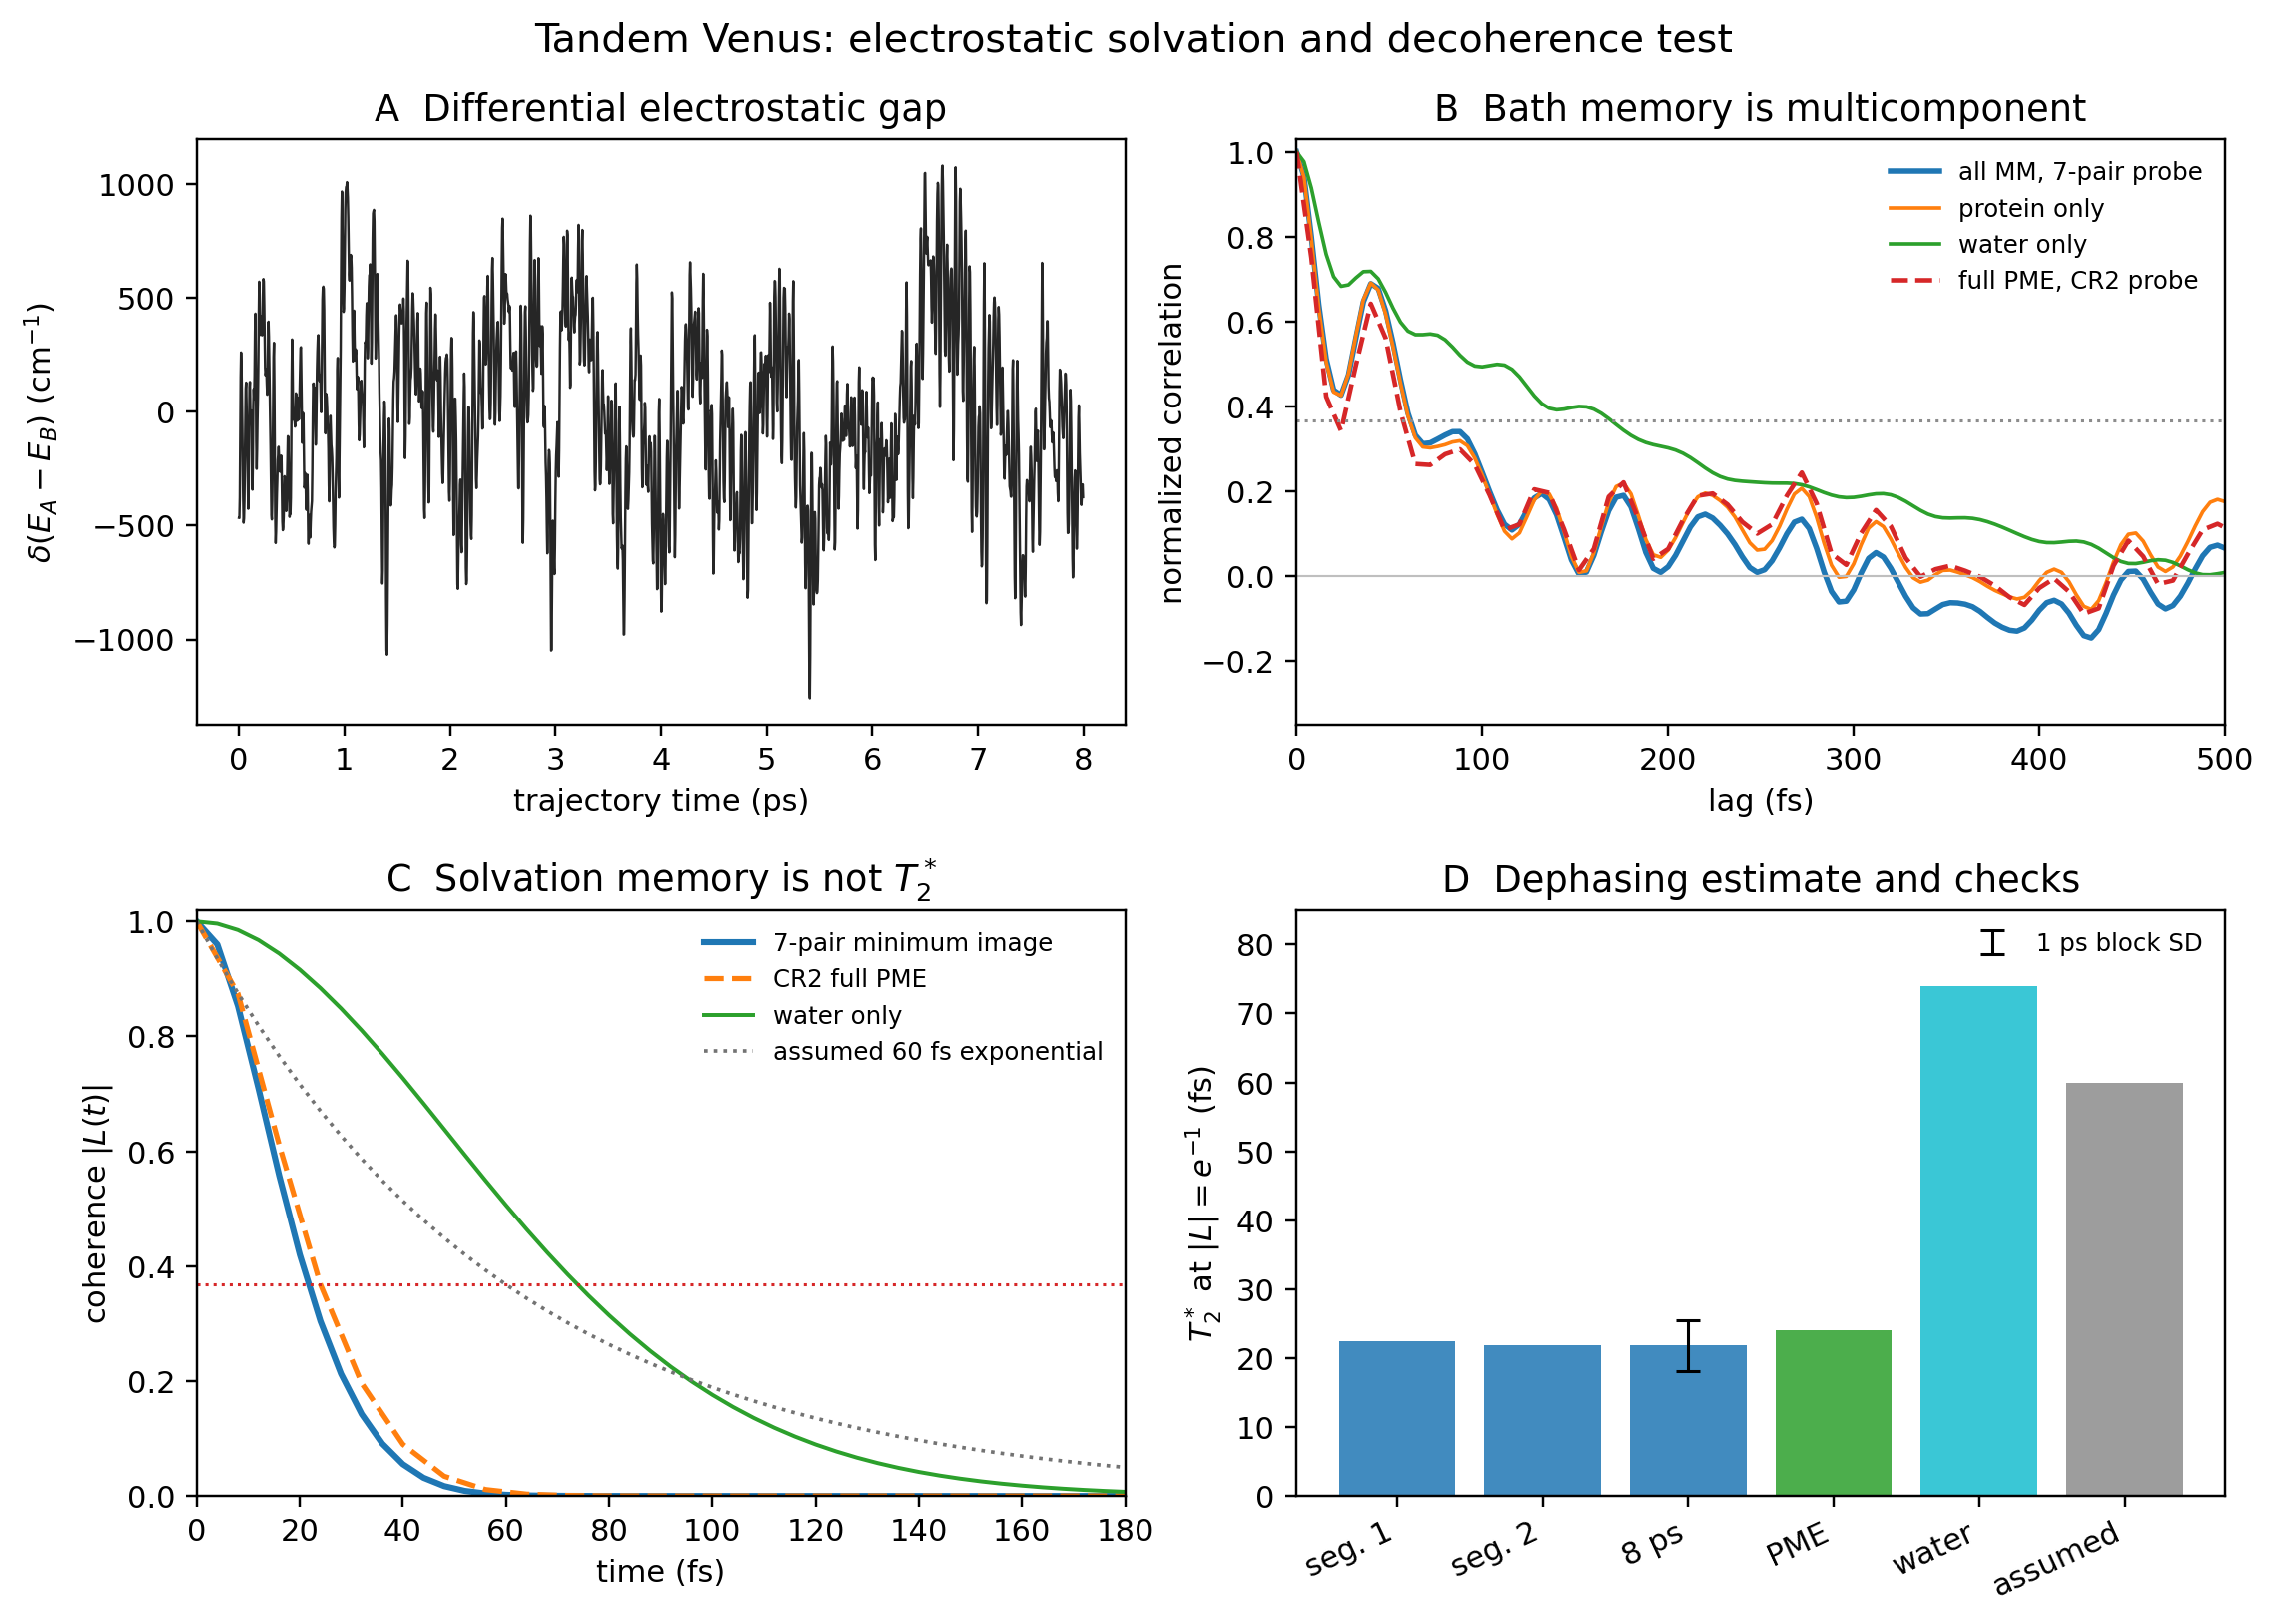
\includegraphics[width=0.79\linewidth]{../solvation_decoherence_test/validation_8ps/solvation_decoherence_validation.png}
  \caption{Project-generated validation summary.  The panels show the
  differential gap, multicomponent correlation, cumulant coherence envelopes,
  and segment/block/PME/component lifetime checks.}
  \label{fig:validation}
\end{figure}

\subsection{Robustness checks}

\begin{table}[ht]
\centering
\caption{Sensitivity and replication checks for the classical cumulant
lifetime.}
\label{tab:robustness}
\small
\begin{tabularx}{\linewidth}{@{}Xl@{}}
\toprule
Check & Result\\
\midrule
Two contiguous 4 ps segments & 22.40 and 21.81 fs\\
Eight independent 1 ps blocks & median 24.52 fs; SD 3.73 fs; range 19.67--29.99 fs\\
Sampling at 4, 8, 16 and 32 fs & 21.80, 22.24, 24.21 and 22.52 fs\\
Remove explicit ions from estimator & 21.80 to 21.62 fs\\
Dominant NTO pair only & 21.95 fs\\
Dipole-matched seven-pair atomic probe & 22.01 fs\\
Full PME cross-check & 24.01 fs\\
PME finite-difference scale halved & 0.00055 $\wn$ RMS trace change\\
\bottomrule
\end{tabularx}
\end{table}

These checks show that the 22--24 fs result is not caused by sampling stride,
one trajectory segment, the small ion contribution, NTO truncation, probe
dipole mismatch or the minimum-image electrostatic kernel.

\section{Spectral sensitivity}

For an exponential homogeneous coherence envelope, the Lorentzian half-width
is
\begin{equation}
  \Gamma_{\mathrm{HWHM}}=\frac{1}{2\pi c\Ttwo}.
\end{equation}
The manuscript's 60 fs reference gives $88.48\ \wn$.  Using the PME lifetime
gives $221.07\ \wn$ (FWHM $442.13\ \wn$), which exceeds the mean Davydov
splitting $2J=234.38\ \wn$ for $J=\Jmean$.  The exciton centres remain at
520.69 and 527.12 nm because changing $\Ttwo$ changes broadening rather than
the coupling.

The CD sign order survives, but its extrema move from 520.60/527.20 nm to
519.47/528.36 nm.  More importantly, the raw peak falls to 0.263 of the 60 fs
value, a 73.7\% reduction.  Independent normalization conceals this loss;
Fig.~\ref{fig:common-scale} therefore uses one common amplitude scale.

\begin{figure}[ht]
  \centering
  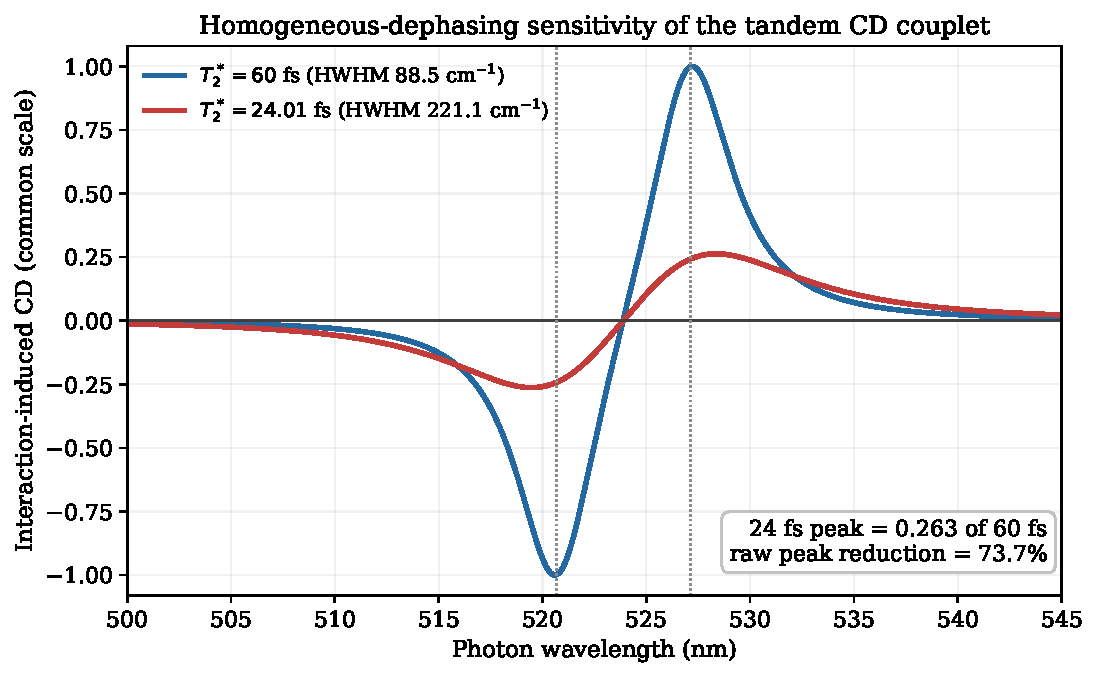
\includegraphics[width=\linewidth]{Fig_T2_CommonScale.pdf}
  \caption{Project-generated 60 fs and 24.01 fs tandem CD differences on a
  shared amplitude scale.  Dotted lines mark the mean exciton centres.  The
  faster-dephasing curve is broader and has only 26.3\% of the raw 60 fs peak.}
  \label{fig:common-scale}
\end{figure}

Under the simple criterion $\mathrm{FWHM}<2J$, the threshold for resolving the
two branches is $\Ttwo=45.3$ fs.  A 22--24 fs Lorentzian lifetime would therefore
not support a resolved linear-absorption doublet, even though the
interaction-induced CD sign topology remains visible.

\section{Relation to the experimental literature}

Nguyen et al.\ report a constrained dVenus apparent coupling of
$130.79\ \wn$ and Lorentzian HWHM parameters of 293.51 and
$439.25\ \wn$ in their three-component difference-CD fit
\cite{nguyen2025}.  The present $J=117.19\pm5.55\ \wn$ is about 10\% lower and
is in good magnitude agreement.  The 24 fs model width is directionally closer
to the experimental fit widths than the 60 fs width, but this is not a direct
validation: the experimental widths also contain inhomogeneous, vibronic and
site-energy contributions absent from the present S1-only model.

Nguyen et al.\ also report a $128.0\pm8.1$ fs coherence time for a dried
dVenus-TD thin film measured with two-pulse near-field microscopy
\cite{nguyen2025}.  That experiment probes an optical ground--excited-state
polarization in a thin film.  The present calculation probes differential
inter-site phase noise in an explicitly solvated dimer.  The samples and
observables differ, so their numerical values must not be equated.

Kim et al.\ observed a room-temperature Venus CD couplet and photon
antibunching, but did not directly measure a Venus $\Ttwo$\cite{kim2019}.  Their
0.44--44 ps range was inferred from an assumed energy-transfer rate and coupling
regime.  The 22--24 fs classical estimate is much shorter than that inference.
It remains compatible with the direct steady-state observation in the limited
sense that vertical absorption occurs on a roughly 1--10 fs timescale and can
imprint an excitonic spectrum before subsequent phase loss.  The calculation
therefore supports rapid optical imprinting while challenging a simple picture
of the beta barrel as a passive source of long-lived coherence: the barrel can
shield common-mode bulk-water fluctuations while its internal protein
electrostatics remain an active differential bath.

\section{Limitations and publication threshold}

\begin{enumerate}
  \item Equation~\eqref{eq:cumulant} uses a classical fixed-charge correlation
        and lacks quantum detailed balance.  It is not a rigorous quantum
        $\Ttwo$.
  \item The probe is a fixed STEOM difference density.  Geometry-dependent
        excitation energies, intrachromophore vibrations, non-Condon effects
        and population relaxation are omitted.
  \item AMBER/TIP3P is non-polarizable; mutual QM/MM induction is absent.
  \item Eight picoseconds resolves the ultrafast decay but cannot converge slow
        protein and solvent modes.
  \item The retained production box is net $-2e$ after transplanting two exact
        $-1$ CR2 parameter sets.  Removing ions changes $\Ttwo$ by only 0.2 fs,
        but a publication-quality calculation should rebuild and neutralize the
        box.
  \item The stable first crossings, block replication and direct coherence
        envelope are preferred over unstable biexponential tail fits.
\end{enumerate}

A publication-quality estimate should compute geometry-dependent
electrostatic-embedding QM/MM gaps on a high-cadence subset, calibrate the
tractable excited-state method against retained STEOM points, construct a
quantum-corrected spectral density, and propagate a non-Markovian lineshape or
reduced-density-matrix model.  Until then, 22--24 fs should be described as a
classical electrostatic sensitivity result.

\section{Reproducibility map}

The difference probe is constructed by
\texttt{build\_steom\_difference\_probe.py}.  Local electrostatic traces and
the classical cumulant are generated by
\texttt{analyze\_solvation\_decoherence.py}; the independent PME derivative is
implemented in \texttt{analyze\_pme\_decoherence.py}; block and stride tests are
performed by \texttt{validate\_solvation\_decoherence.py}; and the validation
summary is drawn by \texttt{plot\_solvation\_validation.py}.  The shared-scale
spectrum in Fig.~\ref{fig:common-scale} is generated by
\texttt{notes/make\_decoherence\_note\_figure.py}.  Compact gap traces,
summaries and audit records accompany these programs.  Full trajectories and
licensed electronic-structure scratch files remain external because of their
size and redistribution constraints.

\begin{thebibliography}{9}
\bibitem{kim2019}
Y. Kim, H. L. Puhl, E. Chen, G. H. Taumoefolau, T. A. Nguyen,
D. S. Kliger, P. S. Blank and S. S. Vogel,
``Venus$_{\mathrm{A206}}$ Dimers Behave Coherently at Room Temperature,''
\emph{Biophysical Journal} \textbf{116}, 1918--1930 (2019),
\href{https://doi.org/10.1016/j.bpj.2019.04.014}{doi:10.1016/j.bpj.2019.04.014}.

\bibitem{nguyen2025}
T. Nguyen, H. L. Puhl, E. Chen, K. Hines, C. Rani, P. S. Blank,
B. Carlotti, Y. Kim, T. Goodson III and S. S. Vogel,
``Anomalous photophysical behaviors attributed to excitonic coupling in
fluorescent proteins,'' \emph{Biophysical Journal} \textbf{124}, 4293--4309
(2025),
\href{https://doi.org/10.1016/j.bpj.2025.10.022}{doi:10.1016/j.bpj.2025.10.022}.
\end{thebibliography}

\end{document}
